\makeatletter \@ifundefined{rootpath}{% Manual to memoir http://mirrors.dotsrc.org/ctan/macros/latex/contrib/memoir/memman.pdf

%\documentclass[a4paper,12pt,fleqn,openany,twoside]{memoir} %two sides for printing
\documentclass[a4paper,12pt,fleqn,openany,oneside]{memoir} %one side for pdf
\usepackage[english]{babel}
\usepackage[utf8]{inputenc}
\usepackage{microtype}
\usepackage{paralist}

%Definitions
\usepackage{amsthm}
\theoremstyle{plain}
\newtheorem{thm}{Theorem}[chapter] % reset theorem numbering for each chapter
\theoremstyle{definition}
\newtheorem{defn}[thm]{Definition}

% Choses the depth of numerations
\setsecnumdepth{subsubsection}

% Choses the depth of toc
%\maxtocdepth{subsection}

% Turn figures sideways with \begin{sideways} figure \end{sideways}
\usepackage{rotating}

% LaTeX logical statements
\usepackage{ifthen}

% Fancy space after use of e.g. command
\usepackage{xspace}

% Skips after paragraphs
\usepackage{parskip}

% Layout settings
\setlength{\parindent}{0cm}
\setlength{\parskip}{2ex plus 2ex} %kan udvides til f.eks: '2ex plus 2ex minus 0ex'

\sloppybottom

% Don't make a collection per default
\newcommand{\worksheetcollection}{false}

% Bibtex
\usepackage[square,numbers,sort,comma]{natbib}
%\usepackage{cite}
%\bibliographystyle{plainnat}
\bibliographystyle{IEEEtran}


% Fixmes
\usepackage{fixme}
\fxsetup{draft}

% Mathematic
\usepackage{amsmath}
\usepackage{amsfonts}
\usepackage{amssymb}
\usepackage{stmaryrd}
\allowdisplaybreaks[1]


% Acronyms
\usepackage[printonlyused]{acronym}

% Images
\usepackage{graphicx}
\usepackage{wrapfig}
\usepackage[outdir=./]{epstopdf}
\usepackage{epsfig}


% Captions ans subcaptions
\captionnamefont{\footnotesize\bfseries}
\captiontitlefont{\footnotesize}

% Enable memoir subfloats for figures and tables
\newsubfloat{figure}
\newsubfloat{table}

% Hack memoir subfigure styles to have bold label and footnotesize fonts
\renewcommand{\thesubfigure}{\footnotesize\bfseries{(\alph{subfigure})}}
\renewcommand{\thesubtable}{\footnotesize\bfseries{(\alph{subtable})}}

\renewcommand{\subcaption}[2][]{\subbottom[\footnotesize{#1}]{#2}}

% Memoir tweak pagenumbers
%\pagestyle{headings}

% Tikz
\usepackage{tikz}
\usetikzlibrary{arrows,shapes,calc,positioning}
\pgfmathsetseed{1}

%Pgf plots
\usepackage{pgfplots}
\pgfplotsset{compat=1.5}
% loatbarrier, keep figures within (sub,subsub) sections
\usepackage{placeins}
\usepackage{pgfplots}
\usepgfplotslibrary{units}
\usepackage[space-before-unit,range-units = repeat]{siunitx}

% Hyperlinked auto references
\usepackage[hidelinks]{hyperref}
\usepackage[nameinlink]{cleveref}
\crefname{lstlisting}{Listing}{Listings}  
\Crefname{lstlisting}{Listing}{Listings}

\crefname{thm}{definition}{definitions}
\Crefname{thm}{Definition}{Definitions}

%\def\chapterautorefname{Kapitel}
%\def\sectionautorefname{Afsnit}
%\def\subsectionautorefname{Afsnit}
%\def\subsubsectionautorefname{Underafsnit}
%\def\figureautorefname{Figur}
%\def\lstlistingautorefname{Listing}
%\def\lstnumberautorefname{Linje}
%\def\itemautorefname{Punkt}
\usepackage[hypcap]{caption} % Link to top of the figure and not the caption

%Sick shit to make \Autoref command
%http://tex.stackexchange.com/questions/36575/autorefs-inserted-text-has-not-the-correct-case
\def\HyLang@english{%
  \def\equationautorefname{Equation}%
  \def\footnoteautorefname{Footnote}%
  \def\itemautorefname{item}%
  \def\figureautorefname{Figure}%
  \def\tableautorefname{Table}%
  \def\partautorefname{Part}%
  \def\appendixautorefname{Appendix}%
  \def\chapterautorefname{Chapter}%
  \def\sectionautorefname{Section}%
  \def\subsectionautorefname{Subsection}%
  \def\subsubsectionautorefname{Subsubsection}%
  \def\paragraphautorefname{Paragraph}%
  \def\subparagraphautorefname{Subparagraph}%
  \def\FancyVerbLineautorefname{Line}%
  \def\theoremautorefname{Theorem}%
  \def\pageautorefname{Page}%
}

% Reference greencommentssections with number and name
\usepackage{nameref}
\newcommand{\bsnameref}[1]{\Cref{#1} ``\nameref{#1}''}
\newcommand{\bsref}[1]{\Cref{#1}}
\newcommand{\bsbilagref}[1]{Appendix \ref{#1}}
\newcommand{\bsbilagnameref}[1]{Appendix \ref{#1} ``\nameref{#1}''}
\newcommand{\pling}[1]{``#1''}


% Listings for code qoutes
\usepackage{listings}
%\usepackage[usenames,dvipsnames,svgnames,table]{xcolor}
\usepackage{color}
\usepackage{xcolor}
\definecolor{bluekeywords}{rgb}{0.13,0.13,1}
\definecolor{greencomments}{rgb}{0,0.5,0}
\definecolor{redstrings}{rgb}{0.9,0,0}
\usepackage{caption} 
\usepackage{multicol}
\DeclareCaptionFont{white}{\color{white}}
\DeclareCaptionFormat{listing}{\colorbox{gray}{\parbox{\textwidth}{#1#2#3}}}
\captionsetup[lstlisting]{format=listing,labelfont=white,textfont=white}
%\lstset{numbers=left}
\usepackage{courier}
\lstset{
	basicstyle=\footnotesize\ttfamily,
	tabsize=2,
	breaklines=true,
  literate={æ}{{\ae}}1 {ø}{{\o}}1 {å}{{\aa}}1 {Æ}{{\AE}}1 {Ø}{{\O}}1 {Å}{{\AA}}1,
  keywords={typeof, new, true, false, catch, function, return, null, catch, switch, var, if, in, while, do, else, case, break},
  keywordstyle=\color{blue}\bfseries,
  ndkeywords={class, export, boolean, throw, implements, import, using, this},
  ndkeywordstyle=\color{darkgray}\bfseries,
  identifierstyle=\color{black},
  sensitive=false,
  comment=[l]{//},
  morecomment=[s]{/*}{*/},
  commentstyle=\color{purple}\ttfamily,
  stringstyle=\color{red}\ttfamily,
  numbers=left,
  numbersep=-5pt,
  showstringspaces=false,
  showspaces=false,
  %morestring=[b]',
  %morestring=[b]"
}
\lstnewenvironment{code}[1][]%
  {\minipage{\linewidth} 
   \lstset{basicstyle=\ttfamily\footnotesize,frame=single,#1}}
  {\endminipage}

\lstdefinelanguage{scala}{
  morekeywords={abstract,case,catch,class,def,%
    do,else,extends,false,final,finally,%
    for,if,implicit,import,match,mixin,%
    new,null,object,override,package,%
    private,protected,requires,return,sealed,%
    super,this,throw,trait,true,try,%
    type,val,var,while,with,yield, Unit, Boolean, Int},
  otherkeywords={=>,<-,<\%,<:,>:,\#,@},
  sensitive=true,
  morecomment=[l]{//},
  morecomment=[n]{/*}{*/},
  morestring=[b]",
  morestring=[b]',
  morestring=[b]"""
}

\lstdefinelanguage{clojure}%
{morekeywords={*,*1,*2,*3,*agent*,*allow-unresolved-vars*,*assert*,*clojure-version*,*command-line-args*,%
*compile-files*,*compile-path*,*e,*err*,*file*,*flush-on-newline*,*in*,*macro-meta*,%
*math-context*,*ns*,*out*,*print-dup*,*print-length*,*print-level*,*print-meta*,*print-readably*,%
*read-eval*,*source-path*,*use-context-classloader*,*warn-on-reflection*,+,-,->,->>,..,/,:else,%
<,<=,=,==,>,>=,@,accessor,aclone,add-classpath,add-watch,agent,agent-errors,aget,alength,alias,%
all-ns,alter,alter-meta!,alter-var-root,amap,ancestors,and,apply,areduce,array-map,aset,%
aset-boolean,aset-byte,aset-char,aset-double,aset-float,aset-int,aset-long,aset-short,assert,%
assoc,assoc!,assoc-in,associative?,atom,await,await-for,await1,bases,bean,bigdec,bigint,binding,%
bit-and,bit-and-not,bit-clear,bit-flip,bit-not,bit-or,bit-set,bit-shift-left,bit-shift-right,%
bit-test,bit-xor,boolean,boolean-array,booleans,bound-fn,bound-fn*,butlast,byte,byte-array,%
bytes,cast,char,char-array,char-escape-string,char-name-string,char?,chars,chunk,chunk-append,%
chunk-buffer,chunk-cons,chunk-first,chunk-next,chunk-rest,chunked-seq?,class,class?,%
clear-agent-errors,clojure-version,coll?,comment,commute,comp,comparator,compare,compare-and-set!,%
compile,complement,concat,cond,condp,conj,conj!,cons,constantly,construct-proxy,contains?,count,%
counted?,create-ns,create-struct,cycle,dec,decimal?,declare,def,definline,defmacro,defmethod,%
defmulti,defn,defn-,defonce,defprotocol,defstruct,deftype,delay,delay?,deliver,deref,derive,%
descendants,destructure,disj,disj!,dissoc,dissoc!,distinct,distinct?,do,do-template,doall,doc,%
dorun,doseq,dosync,dotimes,doto,double,double-array,doubles,drop,drop-last,drop-while,empty,empty?,%
ensure,enumeration-seq,eval,even?,every?,false,false?,ffirst,file-seq,filter,finally,find,find-doc,%
find-ns,find-var,first,float,float-array,float?,floats,flush,fn,fn?,fnext,for,force,format,future,%
future-call,future-cancel,future-cancelled?,future-done?,future?,gen-class,gen-interface,gensym,%
get,get-in,get-method,get-proxy-class,get-thread-bindings,get-validator,hash,hash-map,hash-set,%
identical?,identity,if,if-let,if-not,ifn?,import,in-ns,inc,init-proxy,instance?,int,int-array,%
integer?,interleave,intern,interpose,into,into-array,ints,io!,isa?,iterate,iterator-seq,juxt,%
key,keys,keyword,keyword?,last,lazy-cat,lazy-seq,let,letfn,line-seq,list,list*,list?,load,load-file,%
load-reader,load-string,loaded-libs,locking,long,long-array,longs,loop,macroexpand,macroexpand-1,%
make-array,make-hierarchy,map,map?,mapcat,max,max-key,memfn,memoize,merge,merge-with,meta,%
method-sig,methods,min,min-key,mod,monitor-enter,monitor-exit,name,namespace,neg?,new,newline,%
next,nfirst,nil,nil?,nnext,not,not-any?,not-empty,not-every?,not=,ns,ns-aliases,ns-imports,%
ns-interns,ns-map,ns-name,ns-publics,ns-refers,ns-resolve,ns-unalias,ns-unmap,nth,nthnext,num,%
number?,odd?,or,parents,partial,partition,pcalls,peek,persistent!,pmap,pop,pop!,pop-thread-bindings,%
pos?,pr,pr-str,prefer-method,prefers,primitives-classnames,print,print-ctor,print-doc,print-dup,%
print-method,print-namespace-doc,print-simple,print-special-doc,print-str,printf,println,println-str,%
prn,prn-str,promise,proxy,proxy-call-with-super,proxy-mappings,proxy-name,proxy-super,%
push-thread-bindings,pvalues,quot,rand,rand-int,range,ratio?,rational?,rationalize,re-find,%
re-groups,re-matcher,re-matches,re-pattern,re-seq,read,read-line,read-string,recur,reduce,ref,%
ref-history-count,ref-max-history,ref-min-history,ref-set,refer,refer-clojure,reify,%
release-pending-sends,rem,remove,remove-method,remove-ns,remove-watch,repeat,repeatedly,%
replace,replicate,require,reset!,reset-meta!,resolve,rest,resultset-seq,reverse,reversible?,%
rseq,rsubseq,second,select-keys,send,send-off,seq,seq?,seque,sequence,sequential?,set,set!,%
set-validator!,set?,short,short-array,shorts,shutdown-agents,slurp,some,sort,sort-by,sorted-map,%
sorted-map-by,sorted-set,sorted-set-by,sorted?,special-form-anchor,special-symbol?,split-at,%
split-with,str,stream?,string?,struct,struct-map,subs,subseq,subvec,supers,swap!,symbol,symbol?,%
sync,syntax-symbol-anchor,take,take-last,take-nth,take-while,test,the-ns,throw,time,to-array,%
to-array-2d,trampoline,transient,tree-seq,true,true?,try,type,unchecked-add,unchecked-dec,%
unchecked-divide,unchecked-inc,unchecked-multiply,unchecked-negate,unchecked-remainder,%
unchecked-subtract,underive,unquote,unquote-splicing,update-in,update-proxy,use,val,vals,%
var,var-get,var-set,var?,vary-meta,vec,vector,vector?,when,when-first,when-let,when-not,%
while,with-bindings,with-bindings*,with-in-str,with-loading-context,with-local-vars,%
with-meta,with-open,with-out-str,with-precision,xml-seq,zero?,zipmap
},%
   sensitive,% ???
   alsodigit=-,%
   morecomment=[l];,%
   morestring=[b]"%
  }[keywords,comments,strings]%

% Worksheet commands
\newcommand{\worksheetstart}[5]{ %Title, Revision, Date, Author, rootpath
	\ifthenelse{\equal{\worksheetcollection}{false}}{
		\newcommand{\rootpath}{#5}
		\documentheader
		\chapter{#1}
	}{
		\chapter{#1}
	}
%	\vspace{-1em}
%	\textbf{\tiny Revision #2 at #3. Written by #4}\\
%	\textbf{\tiny Hovedansvarlig #4}\\
%	\vspace{2em}\\
}

\newcommand{\worksheetend}{
	\ifthenelse{\equal{\worksheetcollection}{false}}{
		\collectionend
	}{}
}

\newcommand{\documentheader}{
	% Draws a tikz camera
% #1 is the coordinate to the top left corner
% #2 is a label for the righthand center position
% #3 is the text shown in the center of the camera
\newcommand{\camera}[3]{
\coordinate (anchor) at #1;
\draw (anchor) -- ($ (anchor) + (0em,-20pt) $) -- ($ (anchor) + (10pt, -15pt) $) -- ($ (anchor) + (10pt,-5pt)$) -- cycle;
\draw ($ (anchor) + (10pt,-5pt) $) -- ($ (anchor) + (10pt,0pt) $) -- ($ (anchor) + (50pt,0pt) $) -- ($ (anchor) + (50pt,-20pt) $) -- node[yshift=10pt] {\tiny #3} ($ (anchor) + (10pt,-20pt) $)-- cycle;
\coordinate (#2) at ($ (anchor) + (50pt,-10pt) $);
}

\newcounter{frameNumber}
\newcommand{\frameWithSize}[3][false]{
	\stepcounter{frameNumber}
	\coordinate (anchor) at #2;
	\ifthenelse{\equal{#1}{false}}{
		\def\frameNumber{\arabic{frameNumber}}
	}{
		\def\frameNumber{#1}
	}
	\pgfmathtruncatemacro\randomnumber{random(0,4)}
	\node[yshift=20pt] at (anchor) {\frameNumber};
	\ifthenelse{\equal{#3}{I}}{
		\node[draw, minimum size=20pt, fill=green!60] at (anchor) {I};
		\filldraw[fill=gray] ($(anchor) + (-10pt,-40pt)$) rectangle ($(anchor) + (10pt,-20pt) + (0pt,\randomnumber pt)$);
	}{
		\ifthenelse{\equal{#3}{P}}{
			\node[draw, minimum size=20pt, fill=yellow!60] at (anchor) {P};
			\filldraw[fill=gray] ($(anchor) + (-10pt,-40pt)$) rectangle ($(anchor) + (10pt,-30pt) + (0pt,\randomnumber pt)$);
		}{
			\node[draw, minimum size=20pt, fill=blue!40!yellow!60!black] at (anchor) {\color{white}B};
			\filldraw[fill=gray] ($(anchor) + (-10pt,-40pt)$) rectangle ($(anchor) + (10pt,-37pt) + (0pt,\randomnumber pt)$);
		}
	}
	\draw[thick] ($(anchor) + (-10pt,-40pt)$) -- +(20pt,0pt);
}

	\begin{document}
	%\renewcommand{\chaptername}{Worksheet}
	\chapterstyle{section}
	\renewcommand{\beforechapskip}{0pt}
	\renewcommand{\afterchapskip}{0pt}
}

\newcommand{\collectionstart}[1]{
	\newcommand{\rootpath}{#1}
	\renewcommand{\worksheetcollection}{true}
	\documentheader
	\frontmatter
	%\forside
	\makeatletter \@ifundefined{rootpath}{% Manual to memoir http://mirrors.dotsrc.org/ctan/macros/latex/contrib/memoir/memman.pdf

%\documentclass[a4paper,12pt,fleqn,openany,twoside]{memoir} %two sides for printing
\documentclass[a4paper,12pt,fleqn,openany,oneside]{memoir} %one side for pdf
\usepackage[english]{babel}
\usepackage[utf8]{inputenc}
\usepackage{microtype}
\usepackage{paralist}

%Definitions
\usepackage{amsthm}
\theoremstyle{plain}
\newtheorem{thm}{Theorem}[chapter] % reset theorem numbering for each chapter
\theoremstyle{definition}
\newtheorem{defn}[thm]{Definition}

% Choses the depth of numerations
\setsecnumdepth{subsubsection}

% Choses the depth of toc
%\maxtocdepth{subsection}

% Turn figures sideways with \begin{sideways} figure \end{sideways}
\usepackage{rotating}

% LaTeX logical statements
\usepackage{ifthen}

% Fancy space after use of e.g. command
\usepackage{xspace}

% Skips after paragraphs
\usepackage{parskip}

% Layout settings
\setlength{\parindent}{0cm}
\setlength{\parskip}{2ex plus 2ex} %kan udvides til f.eks: '2ex plus 2ex minus 0ex'

\sloppybottom

% Don't make a collection per default
\newcommand{\worksheetcollection}{false}

% Bibtex
\usepackage[square,numbers,sort,comma]{natbib}
%\usepackage{cite}
%\bibliographystyle{plainnat}
\bibliographystyle{IEEEtran}


% Fixmes
\usepackage{fixme}
\fxsetup{draft}

% Mathematic
\usepackage{amsmath}
\usepackage{amsfonts}
\usepackage{amssymb}
\usepackage{stmaryrd}
\allowdisplaybreaks[1]


% Acronyms
\usepackage[printonlyused]{acronym}

% Images
\usepackage{graphicx}
\usepackage{wrapfig}
\usepackage[outdir=./]{epstopdf}
\usepackage{epsfig}


% Captions ans subcaptions
\captionnamefont{\footnotesize\bfseries}
\captiontitlefont{\footnotesize}

% Enable memoir subfloats for figures and tables
\newsubfloat{figure}
\newsubfloat{table}

% Hack memoir subfigure styles to have bold label and footnotesize fonts
\renewcommand{\thesubfigure}{\footnotesize\bfseries{(\alph{subfigure})}}
\renewcommand{\thesubtable}{\footnotesize\bfseries{(\alph{subtable})}}

\renewcommand{\subcaption}[2][]{\subbottom[\footnotesize{#1}]{#2}}

% Memoir tweak pagenumbers
%\pagestyle{headings}

% Tikz
\usepackage{tikz}
\usetikzlibrary{arrows,shapes,calc,positioning}
\pgfmathsetseed{1}

%Pgf plots
\usepackage{pgfplots}
\pgfplotsset{compat=1.5}
% loatbarrier, keep figures within (sub,subsub) sections
\usepackage{placeins}
\usepackage{pgfplots}
\usepgfplotslibrary{units}
\usepackage[space-before-unit,range-units = repeat]{siunitx}

% Hyperlinked auto references
\usepackage[hidelinks]{hyperref}
\usepackage[nameinlink]{cleveref}
\crefname{lstlisting}{Listing}{Listings}  
\Crefname{lstlisting}{Listing}{Listings}

\crefname{thm}{definition}{definitions}
\Crefname{thm}{Definition}{Definitions}

%\def\chapterautorefname{Kapitel}
%\def\sectionautorefname{Afsnit}
%\def\subsectionautorefname{Afsnit}
%\def\subsubsectionautorefname{Underafsnit}
%\def\figureautorefname{Figur}
%\def\lstlistingautorefname{Listing}
%\def\lstnumberautorefname{Linje}
%\def\itemautorefname{Punkt}
\usepackage[hypcap]{caption} % Link to top of the figure and not the caption

%Sick shit to make \Autoref command
%http://tex.stackexchange.com/questions/36575/autorefs-inserted-text-has-not-the-correct-case
\def\HyLang@english{%
  \def\equationautorefname{Equation}%
  \def\footnoteautorefname{Footnote}%
  \def\itemautorefname{item}%
  \def\figureautorefname{Figure}%
  \def\tableautorefname{Table}%
  \def\partautorefname{Part}%
  \def\appendixautorefname{Appendix}%
  \def\chapterautorefname{Chapter}%
  \def\sectionautorefname{Section}%
  \def\subsectionautorefname{Subsection}%
  \def\subsubsectionautorefname{Subsubsection}%
  \def\paragraphautorefname{Paragraph}%
  \def\subparagraphautorefname{Subparagraph}%
  \def\FancyVerbLineautorefname{Line}%
  \def\theoremautorefname{Theorem}%
  \def\pageautorefname{Page}%
}

% Reference greencommentssections with number and name
\usepackage{nameref}
\newcommand{\bsnameref}[1]{\Cref{#1} ``\nameref{#1}''}
\newcommand{\bsref}[1]{\Cref{#1}}
\newcommand{\bsbilagref}[1]{Appendix \ref{#1}}
\newcommand{\bsbilagnameref}[1]{Appendix \ref{#1} ``\nameref{#1}''}
\newcommand{\pling}[1]{``#1''}


% Listings for code qoutes
\usepackage{listings}
%\usepackage[usenames,dvipsnames,svgnames,table]{xcolor}
\usepackage{color}
\usepackage{xcolor}
\definecolor{bluekeywords}{rgb}{0.13,0.13,1}
\definecolor{greencomments}{rgb}{0,0.5,0}
\definecolor{redstrings}{rgb}{0.9,0,0}
\usepackage{caption} 
\usepackage{multicol}
\DeclareCaptionFont{white}{\color{white}}
\DeclareCaptionFormat{listing}{\colorbox{gray}{\parbox{\textwidth}{#1#2#3}}}
\captionsetup[lstlisting]{format=listing,labelfont=white,textfont=white}
%\lstset{numbers=left}
\usepackage{courier}
\lstset{
	basicstyle=\footnotesize\ttfamily,
	tabsize=2,
	breaklines=true,
  literate={æ}{{\ae}}1 {ø}{{\o}}1 {å}{{\aa}}1 {Æ}{{\AE}}1 {Ø}{{\O}}1 {Å}{{\AA}}1,
  keywords={typeof, new, true, false, catch, function, return, null, catch, switch, var, if, in, while, do, else, case, break},
  keywordstyle=\color{blue}\bfseries,
  ndkeywords={class, export, boolean, throw, implements, import, using, this},
  ndkeywordstyle=\color{darkgray}\bfseries,
  identifierstyle=\color{black},
  sensitive=false,
  comment=[l]{//},
  morecomment=[s]{/*}{*/},
  commentstyle=\color{purple}\ttfamily,
  stringstyle=\color{red}\ttfamily,
  numbers=left,
  numbersep=-5pt,
  showstringspaces=false,
  showspaces=false,
  %morestring=[b]',
  %morestring=[b]"
}
\lstnewenvironment{code}[1][]%
  {\minipage{\linewidth} 
   \lstset{basicstyle=\ttfamily\footnotesize,frame=single,#1}}
  {\endminipage}

\lstdefinelanguage{scala}{
  morekeywords={abstract,case,catch,class,def,%
    do,else,extends,false,final,finally,%
    for,if,implicit,import,match,mixin,%
    new,null,object,override,package,%
    private,protected,requires,return,sealed,%
    super,this,throw,trait,true,try,%
    type,val,var,while,with,yield, Unit, Boolean, Int},
  otherkeywords={=>,<-,<\%,<:,>:,\#,@},
  sensitive=true,
  morecomment=[l]{//},
  morecomment=[n]{/*}{*/},
  morestring=[b]",
  morestring=[b]',
  morestring=[b]"""
}

\lstdefinelanguage{clojure}%
{morekeywords={*,*1,*2,*3,*agent*,*allow-unresolved-vars*,*assert*,*clojure-version*,*command-line-args*,%
*compile-files*,*compile-path*,*e,*err*,*file*,*flush-on-newline*,*in*,*macro-meta*,%
*math-context*,*ns*,*out*,*print-dup*,*print-length*,*print-level*,*print-meta*,*print-readably*,%
*read-eval*,*source-path*,*use-context-classloader*,*warn-on-reflection*,+,-,->,->>,..,/,:else,%
<,<=,=,==,>,>=,@,accessor,aclone,add-classpath,add-watch,agent,agent-errors,aget,alength,alias,%
all-ns,alter,alter-meta!,alter-var-root,amap,ancestors,and,apply,areduce,array-map,aset,%
aset-boolean,aset-byte,aset-char,aset-double,aset-float,aset-int,aset-long,aset-short,assert,%
assoc,assoc!,assoc-in,associative?,atom,await,await-for,await1,bases,bean,bigdec,bigint,binding,%
bit-and,bit-and-not,bit-clear,bit-flip,bit-not,bit-or,bit-set,bit-shift-left,bit-shift-right,%
bit-test,bit-xor,boolean,boolean-array,booleans,bound-fn,bound-fn*,butlast,byte,byte-array,%
bytes,cast,char,char-array,char-escape-string,char-name-string,char?,chars,chunk,chunk-append,%
chunk-buffer,chunk-cons,chunk-first,chunk-next,chunk-rest,chunked-seq?,class,class?,%
clear-agent-errors,clojure-version,coll?,comment,commute,comp,comparator,compare,compare-and-set!,%
compile,complement,concat,cond,condp,conj,conj!,cons,constantly,construct-proxy,contains?,count,%
counted?,create-ns,create-struct,cycle,dec,decimal?,declare,def,definline,defmacro,defmethod,%
defmulti,defn,defn-,defonce,defprotocol,defstruct,deftype,delay,delay?,deliver,deref,derive,%
descendants,destructure,disj,disj!,dissoc,dissoc!,distinct,distinct?,do,do-template,doall,doc,%
dorun,doseq,dosync,dotimes,doto,double,double-array,doubles,drop,drop-last,drop-while,empty,empty?,%
ensure,enumeration-seq,eval,even?,every?,false,false?,ffirst,file-seq,filter,finally,find,find-doc,%
find-ns,find-var,first,float,float-array,float?,floats,flush,fn,fn?,fnext,for,force,format,future,%
future-call,future-cancel,future-cancelled?,future-done?,future?,gen-class,gen-interface,gensym,%
get,get-in,get-method,get-proxy-class,get-thread-bindings,get-validator,hash,hash-map,hash-set,%
identical?,identity,if,if-let,if-not,ifn?,import,in-ns,inc,init-proxy,instance?,int,int-array,%
integer?,interleave,intern,interpose,into,into-array,ints,io!,isa?,iterate,iterator-seq,juxt,%
key,keys,keyword,keyword?,last,lazy-cat,lazy-seq,let,letfn,line-seq,list,list*,list?,load,load-file,%
load-reader,load-string,loaded-libs,locking,long,long-array,longs,loop,macroexpand,macroexpand-1,%
make-array,make-hierarchy,map,map?,mapcat,max,max-key,memfn,memoize,merge,merge-with,meta,%
method-sig,methods,min,min-key,mod,monitor-enter,monitor-exit,name,namespace,neg?,new,newline,%
next,nfirst,nil,nil?,nnext,not,not-any?,not-empty,not-every?,not=,ns,ns-aliases,ns-imports,%
ns-interns,ns-map,ns-name,ns-publics,ns-refers,ns-resolve,ns-unalias,ns-unmap,nth,nthnext,num,%
number?,odd?,or,parents,partial,partition,pcalls,peek,persistent!,pmap,pop,pop!,pop-thread-bindings,%
pos?,pr,pr-str,prefer-method,prefers,primitives-classnames,print,print-ctor,print-doc,print-dup,%
print-method,print-namespace-doc,print-simple,print-special-doc,print-str,printf,println,println-str,%
prn,prn-str,promise,proxy,proxy-call-with-super,proxy-mappings,proxy-name,proxy-super,%
push-thread-bindings,pvalues,quot,rand,rand-int,range,ratio?,rational?,rationalize,re-find,%
re-groups,re-matcher,re-matches,re-pattern,re-seq,read,read-line,read-string,recur,reduce,ref,%
ref-history-count,ref-max-history,ref-min-history,ref-set,refer,refer-clojure,reify,%
release-pending-sends,rem,remove,remove-method,remove-ns,remove-watch,repeat,repeatedly,%
replace,replicate,require,reset!,reset-meta!,resolve,rest,resultset-seq,reverse,reversible?,%
rseq,rsubseq,second,select-keys,send,send-off,seq,seq?,seque,sequence,sequential?,set,set!,%
set-validator!,set?,short,short-array,shorts,shutdown-agents,slurp,some,sort,sort-by,sorted-map,%
sorted-map-by,sorted-set,sorted-set-by,sorted?,special-form-anchor,special-symbol?,split-at,%
split-with,str,stream?,string?,struct,struct-map,subs,subseq,subvec,supers,swap!,symbol,symbol?,%
sync,syntax-symbol-anchor,take,take-last,take-nth,take-while,test,the-ns,throw,time,to-array,%
to-array-2d,trampoline,transient,tree-seq,true,true?,try,type,unchecked-add,unchecked-dec,%
unchecked-divide,unchecked-inc,unchecked-multiply,unchecked-negate,unchecked-remainder,%
unchecked-subtract,underive,unquote,unquote-splicing,update-in,update-proxy,use,val,vals,%
var,var-get,var-set,var?,vary-meta,vec,vector,vector?,when,when-first,when-let,when-not,%
while,with-bindings,with-bindings*,with-in-str,with-loading-context,with-local-vars,%
with-meta,with-open,with-out-str,with-precision,xml-seq,zero?,zipmap
},%
   sensitive,% ???
   alsodigit=-,%
   morecomment=[l];,%
   morestring=[b]"%
  }[keywords,comments,strings]%

% Worksheet commands
\newcommand{\worksheetstart}[5]{ %Title, Revision, Date, Author, rootpath
	\ifthenelse{\equal{\worksheetcollection}{false}}{
		\newcommand{\rootpath}{#5}
		\documentheader
		\chapter{#1}
	}{
		\chapter{#1}
	}
%	\vspace{-1em}
%	\textbf{\tiny Revision #2 at #3. Written by #4}\\
%	\textbf{\tiny Hovedansvarlig #4}\\
%	\vspace{2em}\\
}

\newcommand{\worksheetend}{
	\ifthenelse{\equal{\worksheetcollection}{false}}{
		\collectionend
	}{}
}

\newcommand{\documentheader}{
	\input{\rootpath/setup/tikz-commands.tex}
	\begin{document}
	%\renewcommand{\chaptername}{Worksheet}
	\chapterstyle{section}
	\renewcommand{\beforechapskip}{0pt}
	\renewcommand{\afterchapskip}{0pt}
}

\newcommand{\collectionstart}[1]{
	\newcommand{\rootpath}{#1}
	\renewcommand{\worksheetcollection}{true}
	\documentheader
	\frontmatter
	%\forside
	\input{\rootpath/worksheets/titlepage/titlepage}
	\input{\rootpath/worksheets/preface/preface}
	%\input{\rootpath/worksheets/forord/forord}
	\newpage
	\newpage
	\tableofcontents*
	\mainmatter
}

\newcommand{\collectionend}{
	\backmatter
	\chapter{List of Acronyms}\vspace{3em}
	\input{\rootpath/setup/acronyms}
	\bibliography{\rootpath/setup/bibliography}
	\end{document}
}


%\newcommand{\bscode}{
%	\lstinline
%}

\font\fontcode=pcrr at 12pt

\newcommand{\bscode}[1]{
	{\fontcode#1}
}



\newcommand{\bscodemath}[1]{
	\text{\lstinline|#1|}
}

\newcommand{\bsqoute}[2]{
	\begin{quote}
		\textit{``#1''}
		\begin{center}
			-- \emph{#2}
		\end{center}
	\end{quote}
}


\newcommand{\lag}{\langle}
\newcommand{\rag}{\rangle}
\newcommand{\besk}[1]{\ensuremath{\lag #1 \rag}}

\newcommand{\namedtodo}[5]
{
  \ifthenelse{\equal{#1}{}}
  {
    \todo[color=#4,caption=
    {\textbf{#3: } #2}]
    {\color{#5}\textbf{#3: }#2}
  }
  {
    \todo[color=#4,caption=
    {\textbf{#3: } #1}
    ,inline]
    {\color{#5}\textbf{#3: }#2}
  }
}
\newcommand{\andreas}[2][]{\namedtodo{#1}{#2}{Andreas}{blue!50!red!10}{black}}
\newcommand{\lone}[2][]{\namedtodo{#1}{#2}{Lone}{orange}{black}}
\definecolor{babypink}{rgb}{0.96, 0.76, 0.76}
\newcommand{\toby}[2][]{\namedtodo{#1}{#2}{Tobias}{babypink}{black}}
\newcommand{\kasper}[2][]{\namedtodo{#1}{#2}{Kasper}{green}{black}}

%multicol
\usepackage{multicol}

% todonotes
%\usepackage[disable]{todonotes} %For final report
\usepackage{todonotes} %For writing notes
\usepackage{fancyvrb}

%Loading AAU macro
\usepackage{lastpage}
%%%%%%%%%%%%%%%%%%%%%%%%%%%%%%%%%%%%%%%%%%%%%%%%
% Macros for the titlepage
%%%%%%%%%%%%%%%%%%%%%%%%%%%%%%%%%%%%%%%%%%%%%%%%
%Creates the aau titlepage
\newcommand{\aautitlepage}[3]{%
  {
    %set up various length
    \ifx\titlepageleftcolumnwidth\undefined
      \newlength{\titlepageleftcolumnwidth}
      \newlength{\titlepagerightcolumnwidth}
    \fi
    \setlength{\titlepageleftcolumnwidth}{0.5\textwidth-\tabcolsep}
    \setlength{\titlepagerightcolumnwidth}{\textwidth-2\tabcolsep-\titlepageleftcolumnwidth}
    %create title page
    \thispagestyle{empty}
    \noindent%
    \begin{tabular}{@{}ll@{}}
      \parbox{\titlepageleftcolumnwidth}{
        \iflanguage{danish}{%
          
\includegraphics[width=\titlepageleftcolumnwidth]{titlepage/figures/aau_logo_da}
        }{%
          
\includegraphics[width=\titlepageleftcolumnwidth]{titlepage/figures/aau_logo_en}
        }
      } &
      \parbox{\titlepagerightcolumnwidth}{\raggedleft\small
        #2
      }\bigskip\\
       #1 &
      \parbox[t]{\titlepagerightcolumnwidth}{%
      \textbf{Abstract:}\bigskip\par
        \fbox{\parbox{\titlepagerightcolumnwidth-2\fboxsep-2\fboxrule}{%
          #3
        }}
      }\\
    \end{tabular}
    \vfill  
    \clearpage
  }
}

% Environment for problem statements
% Can be auto referenced.
\newtheorem{problem}{Problem}
\def\problemautorefname{Problem}

%Create english project info
\newcommand{\englishprojectinfo}[6]{%
  \parbox[t]{\titlepageleftcolumnwidth}{
    \textbf{Title:}\\ #1\bigskip\par
    %\textbf{Theme:}\\ #2\bigskip\par
    \textbf{Project Period:}\\ #2\bigskip\par
    \textbf{Project Group:}\\ #3\bigskip\par
    \textbf{Participants:}\\ #4\bigskip\par
    \textbf{Supervisor:}\\ #5\bigskip\par
    %\textbf{Copies:} #6\bigskip\par
    \textbf{Page Numbers:} \pageref{LastPage}\bigskip\par
    \textbf{Date of Completion:}\\ #6
  }
}



%Create danish project info
%\newcommand{\danishprojectinfo}[7]{%
 % \parbox[t]{\titlepageleftcolumnwidth}{
 %   \textbf{Titel:}\\ #1\bigskip\par
%    %\textbf{Tema:}\\ #2\bigskip\par
%    \textbf{Projektperiode:}\\ #2\bigskip\par
%    \textbf{Projektgruppe:}\\ #4\bigskip\par
%    \textbf{Deltager(e):}\\ #5\bigskip\par
 %   \textbf{Vejleder(e):}\\ #6\bigskip\par
%    \textbf{Oplagstal:} #7\bigskip\par
   % \textbf{Sidetal:} \pageref{LastPage}\bigskip\par
  %  \textbf{Afleveringsdato:}\\ #8
 % }
%}


%roman numerals
%\newcommand*{\rom}[1]{\expandafter\@slowromancap\romannumeral #1@}
\newcommand{\rom}[1]{\uppercase\expandafter{\romannumeral #1\relax}}

%Hypothesis
\newtheorem{hypo}{Hypothesis}

%STM name
\newcommand{\stmname}{AtomiC\#}
\newcommand{\stmnamesp}{AtomiC\# }

}\makeatother
%\worksheetstart{Titlepage}{0}{December 31, 2012}{../../}
\begin{titlingpage}
\aautitlepage{%
  \englishprojectinfo{
    Language Integrated STM in C\# Using the Roslyn Compiler - An Alternative to Locking. %title
    %STM Integration in C\# and the Roslyn Compiler. %title
  }{%
    Spring Semester 2015 %project period
  }{%
    dpt109f15  % project group
  }{%
    %list of group members
    Tobias Ugleholdt Hansen\\
    Andreas Pørtner Karlsen\\ 
    Kasper Breinholt Laurberg\\
  }{%
    %list of supervisors
     Lone Leth Thomsen
  }{%
    \today % date of completion
  }%
}{%department and address
  \textbf{Department of Computer Science}\\
  Selma Lagerløfs Vej 300\\
  DK-9220 Aalborg Ø\\
  \href{http://www.cs.aau.dk}{http://www.cs.aau.dk}
}{% the abstract
% Our motivation
% What have we done
% How did we do it
% Our contribution
This master thesis investigates whether language integrated STM, in terms of usability, is a valid alternative to locking and provides additional benefits compared to library-based STM. In order to do so, an extension of C\# called \stmname has been implemented. \stmname extends C\# with language integrated support for STM, including conditional synchronization using the retry and orelse constructs as well as nesting of transactions.

\stmname was implemented by extending the open source Roslyn C\# compiler. To power \stmname a library-based STM system, based on the TL\rom{2} algorithm, was implemented. The extended Roslyn C\# compiler transforms \stmname source code to regular C\# code which utilizes the STM library. For each of the concurrency approaches: \stmname, library-based STM and locking in C\#, four different concurrency problems, representing different aspects of concurrent programming were implemented. These implementations were analyzed according to a set of usability characteristics facilitating a conclusion upon the usability of language integrated STM in the context of C\#. Our evaluation concludes that \stmname is a valid alternative to locking, and provides better usability than library based STM.}
\end{titlingpage}
	\makeatletter \@ifundefined{rootpath}{% Manual to memoir http://mirrors.dotsrc.org/ctan/macros/latex/contrib/memoir/memman.pdf

%\documentclass[a4paper,12pt,fleqn,openany,twoside]{memoir} %two sides for printing
\documentclass[a4paper,12pt,fleqn,openany,oneside]{memoir} %one side for pdf
\usepackage[english]{babel}
\usepackage[utf8]{inputenc}
\usepackage{microtype}
\usepackage{paralist}

%Definitions
\usepackage{amsthm}
\theoremstyle{plain}
\newtheorem{thm}{Theorem}[chapter] % reset theorem numbering for each chapter
\theoremstyle{definition}
\newtheorem{defn}[thm]{Definition}

% Choses the depth of numerations
\setsecnumdepth{subsubsection}

% Choses the depth of toc
%\maxtocdepth{subsection}

% Turn figures sideways with \begin{sideways} figure \end{sideways}
\usepackage{rotating}

% LaTeX logical statements
\usepackage{ifthen}

% Fancy space after use of e.g. command
\usepackage{xspace}

% Skips after paragraphs
\usepackage{parskip}

% Layout settings
\setlength{\parindent}{0cm}
\setlength{\parskip}{2ex plus 2ex} %kan udvides til f.eks: '2ex plus 2ex minus 0ex'

\sloppybottom

% Don't make a collection per default
\newcommand{\worksheetcollection}{false}

% Bibtex
\usepackage[square,numbers,sort,comma]{natbib}
%\usepackage{cite}
%\bibliographystyle{plainnat}
\bibliographystyle{IEEEtran}


% Fixmes
\usepackage{fixme}
\fxsetup{draft}

% Mathematic
\usepackage{amsmath}
\usepackage{amsfonts}
\usepackage{amssymb}
\usepackage{stmaryrd}
\allowdisplaybreaks[1]


% Acronyms
\usepackage[printonlyused]{acronym}

% Images
\usepackage{graphicx}
\usepackage{wrapfig}
\usepackage[outdir=./]{epstopdf}
\usepackage{epsfig}


% Captions ans subcaptions
\captionnamefont{\footnotesize\bfseries}
\captiontitlefont{\footnotesize}

% Enable memoir subfloats for figures and tables
\newsubfloat{figure}
\newsubfloat{table}

% Hack memoir subfigure styles to have bold label and footnotesize fonts
\renewcommand{\thesubfigure}{\footnotesize\bfseries{(\alph{subfigure})}}
\renewcommand{\thesubtable}{\footnotesize\bfseries{(\alph{subtable})}}

\renewcommand{\subcaption}[2][]{\subbottom[\footnotesize{#1}]{#2}}

% Memoir tweak pagenumbers
%\pagestyle{headings}

% Tikz
\usepackage{tikz}
\usetikzlibrary{arrows,shapes,calc,positioning}
\pgfmathsetseed{1}

%Pgf plots
\usepackage{pgfplots}
\pgfplotsset{compat=1.5}
% loatbarrier, keep figures within (sub,subsub) sections
\usepackage{placeins}
\usepackage{pgfplots}
\usepgfplotslibrary{units}
\usepackage[space-before-unit,range-units = repeat]{siunitx}

% Hyperlinked auto references
\usepackage[hidelinks]{hyperref}
\usepackage[nameinlink]{cleveref}
\crefname{lstlisting}{Listing}{Listings}  
\Crefname{lstlisting}{Listing}{Listings}

\crefname{thm}{definition}{definitions}
\Crefname{thm}{Definition}{Definitions}

%\def\chapterautorefname{Kapitel}
%\def\sectionautorefname{Afsnit}
%\def\subsectionautorefname{Afsnit}
%\def\subsubsectionautorefname{Underafsnit}
%\def\figureautorefname{Figur}
%\def\lstlistingautorefname{Listing}
%\def\lstnumberautorefname{Linje}
%\def\itemautorefname{Punkt}
\usepackage[hypcap]{caption} % Link to top of the figure and not the caption

%Sick shit to make \Autoref command
%http://tex.stackexchange.com/questions/36575/autorefs-inserted-text-has-not-the-correct-case
\def\HyLang@english{%
  \def\equationautorefname{Equation}%
  \def\footnoteautorefname{Footnote}%
  \def\itemautorefname{item}%
  \def\figureautorefname{Figure}%
  \def\tableautorefname{Table}%
  \def\partautorefname{Part}%
  \def\appendixautorefname{Appendix}%
  \def\chapterautorefname{Chapter}%
  \def\sectionautorefname{Section}%
  \def\subsectionautorefname{Subsection}%
  \def\subsubsectionautorefname{Subsubsection}%
  \def\paragraphautorefname{Paragraph}%
  \def\subparagraphautorefname{Subparagraph}%
  \def\FancyVerbLineautorefname{Line}%
  \def\theoremautorefname{Theorem}%
  \def\pageautorefname{Page}%
}

% Reference greencommentssections with number and name
\usepackage{nameref}
\newcommand{\bsnameref}[1]{\Cref{#1} ``\nameref{#1}''}
\newcommand{\bsref}[1]{\Cref{#1}}
\newcommand{\bsbilagref}[1]{Appendix \ref{#1}}
\newcommand{\bsbilagnameref}[1]{Appendix \ref{#1} ``\nameref{#1}''}
\newcommand{\pling}[1]{``#1''}


% Listings for code qoutes
\usepackage{listings}
%\usepackage[usenames,dvipsnames,svgnames,table]{xcolor}
\usepackage{color}
\usepackage{xcolor}
\definecolor{bluekeywords}{rgb}{0.13,0.13,1}
\definecolor{greencomments}{rgb}{0,0.5,0}
\definecolor{redstrings}{rgb}{0.9,0,0}
\usepackage{caption} 
\usepackage{multicol}
\DeclareCaptionFont{white}{\color{white}}
\DeclareCaptionFormat{listing}{\colorbox{gray}{\parbox{\textwidth}{#1#2#3}}}
\captionsetup[lstlisting]{format=listing,labelfont=white,textfont=white}
%\lstset{numbers=left}
\usepackage{courier}
\lstset{
	basicstyle=\footnotesize\ttfamily,
	tabsize=2,
	breaklines=true,
  literate={æ}{{\ae}}1 {ø}{{\o}}1 {å}{{\aa}}1 {Æ}{{\AE}}1 {Ø}{{\O}}1 {Å}{{\AA}}1,
  keywords={typeof, new, true, false, catch, function, return, null, catch, switch, var, if, in, while, do, else, case, break},
  keywordstyle=\color{blue}\bfseries,
  ndkeywords={class, export, boolean, throw, implements, import, using, this},
  ndkeywordstyle=\color{darkgray}\bfseries,
  identifierstyle=\color{black},
  sensitive=false,
  comment=[l]{//},
  morecomment=[s]{/*}{*/},
  commentstyle=\color{purple}\ttfamily,
  stringstyle=\color{red}\ttfamily,
  numbers=left,
  numbersep=-5pt,
  showstringspaces=false,
  showspaces=false,
  %morestring=[b]',
  %morestring=[b]"
}
\lstnewenvironment{code}[1][]%
  {\minipage{\linewidth} 
   \lstset{basicstyle=\ttfamily\footnotesize,frame=single,#1}}
  {\endminipage}

\lstdefinelanguage{scala}{
  morekeywords={abstract,case,catch,class,def,%
    do,else,extends,false,final,finally,%
    for,if,implicit,import,match,mixin,%
    new,null,object,override,package,%
    private,protected,requires,return,sealed,%
    super,this,throw,trait,true,try,%
    type,val,var,while,with,yield, Unit, Boolean, Int},
  otherkeywords={=>,<-,<\%,<:,>:,\#,@},
  sensitive=true,
  morecomment=[l]{//},
  morecomment=[n]{/*}{*/},
  morestring=[b]",
  morestring=[b]',
  morestring=[b]"""
}

\lstdefinelanguage{clojure}%
{morekeywords={*,*1,*2,*3,*agent*,*allow-unresolved-vars*,*assert*,*clojure-version*,*command-line-args*,%
*compile-files*,*compile-path*,*e,*err*,*file*,*flush-on-newline*,*in*,*macro-meta*,%
*math-context*,*ns*,*out*,*print-dup*,*print-length*,*print-level*,*print-meta*,*print-readably*,%
*read-eval*,*source-path*,*use-context-classloader*,*warn-on-reflection*,+,-,->,->>,..,/,:else,%
<,<=,=,==,>,>=,@,accessor,aclone,add-classpath,add-watch,agent,agent-errors,aget,alength,alias,%
all-ns,alter,alter-meta!,alter-var-root,amap,ancestors,and,apply,areduce,array-map,aset,%
aset-boolean,aset-byte,aset-char,aset-double,aset-float,aset-int,aset-long,aset-short,assert,%
assoc,assoc!,assoc-in,associative?,atom,await,await-for,await1,bases,bean,bigdec,bigint,binding,%
bit-and,bit-and-not,bit-clear,bit-flip,bit-not,bit-or,bit-set,bit-shift-left,bit-shift-right,%
bit-test,bit-xor,boolean,boolean-array,booleans,bound-fn,bound-fn*,butlast,byte,byte-array,%
bytes,cast,char,char-array,char-escape-string,char-name-string,char?,chars,chunk,chunk-append,%
chunk-buffer,chunk-cons,chunk-first,chunk-next,chunk-rest,chunked-seq?,class,class?,%
clear-agent-errors,clojure-version,coll?,comment,commute,comp,comparator,compare,compare-and-set!,%
compile,complement,concat,cond,condp,conj,conj!,cons,constantly,construct-proxy,contains?,count,%
counted?,create-ns,create-struct,cycle,dec,decimal?,declare,def,definline,defmacro,defmethod,%
defmulti,defn,defn-,defonce,defprotocol,defstruct,deftype,delay,delay?,deliver,deref,derive,%
descendants,destructure,disj,disj!,dissoc,dissoc!,distinct,distinct?,do,do-template,doall,doc,%
dorun,doseq,dosync,dotimes,doto,double,double-array,doubles,drop,drop-last,drop-while,empty,empty?,%
ensure,enumeration-seq,eval,even?,every?,false,false?,ffirst,file-seq,filter,finally,find,find-doc,%
find-ns,find-var,first,float,float-array,float?,floats,flush,fn,fn?,fnext,for,force,format,future,%
future-call,future-cancel,future-cancelled?,future-done?,future?,gen-class,gen-interface,gensym,%
get,get-in,get-method,get-proxy-class,get-thread-bindings,get-validator,hash,hash-map,hash-set,%
identical?,identity,if,if-let,if-not,ifn?,import,in-ns,inc,init-proxy,instance?,int,int-array,%
integer?,interleave,intern,interpose,into,into-array,ints,io!,isa?,iterate,iterator-seq,juxt,%
key,keys,keyword,keyword?,last,lazy-cat,lazy-seq,let,letfn,line-seq,list,list*,list?,load,load-file,%
load-reader,load-string,loaded-libs,locking,long,long-array,longs,loop,macroexpand,macroexpand-1,%
make-array,make-hierarchy,map,map?,mapcat,max,max-key,memfn,memoize,merge,merge-with,meta,%
method-sig,methods,min,min-key,mod,monitor-enter,monitor-exit,name,namespace,neg?,new,newline,%
next,nfirst,nil,nil?,nnext,not,not-any?,not-empty,not-every?,not=,ns,ns-aliases,ns-imports,%
ns-interns,ns-map,ns-name,ns-publics,ns-refers,ns-resolve,ns-unalias,ns-unmap,nth,nthnext,num,%
number?,odd?,or,parents,partial,partition,pcalls,peek,persistent!,pmap,pop,pop!,pop-thread-bindings,%
pos?,pr,pr-str,prefer-method,prefers,primitives-classnames,print,print-ctor,print-doc,print-dup,%
print-method,print-namespace-doc,print-simple,print-special-doc,print-str,printf,println,println-str,%
prn,prn-str,promise,proxy,proxy-call-with-super,proxy-mappings,proxy-name,proxy-super,%
push-thread-bindings,pvalues,quot,rand,rand-int,range,ratio?,rational?,rationalize,re-find,%
re-groups,re-matcher,re-matches,re-pattern,re-seq,read,read-line,read-string,recur,reduce,ref,%
ref-history-count,ref-max-history,ref-min-history,ref-set,refer,refer-clojure,reify,%
release-pending-sends,rem,remove,remove-method,remove-ns,remove-watch,repeat,repeatedly,%
replace,replicate,require,reset!,reset-meta!,resolve,rest,resultset-seq,reverse,reversible?,%
rseq,rsubseq,second,select-keys,send,send-off,seq,seq?,seque,sequence,sequential?,set,set!,%
set-validator!,set?,short,short-array,shorts,shutdown-agents,slurp,some,sort,sort-by,sorted-map,%
sorted-map-by,sorted-set,sorted-set-by,sorted?,special-form-anchor,special-symbol?,split-at,%
split-with,str,stream?,string?,struct,struct-map,subs,subseq,subvec,supers,swap!,symbol,symbol?,%
sync,syntax-symbol-anchor,take,take-last,take-nth,take-while,test,the-ns,throw,time,to-array,%
to-array-2d,trampoline,transient,tree-seq,true,true?,try,type,unchecked-add,unchecked-dec,%
unchecked-divide,unchecked-inc,unchecked-multiply,unchecked-negate,unchecked-remainder,%
unchecked-subtract,underive,unquote,unquote-splicing,update-in,update-proxy,use,val,vals,%
var,var-get,var-set,var?,vary-meta,vec,vector,vector?,when,when-first,when-let,when-not,%
while,with-bindings,with-bindings*,with-in-str,with-loading-context,with-local-vars,%
with-meta,with-open,with-out-str,with-precision,xml-seq,zero?,zipmap
},%
   sensitive,% ???
   alsodigit=-,%
   morecomment=[l];,%
   morestring=[b]"%
  }[keywords,comments,strings]%

% Worksheet commands
\newcommand{\worksheetstart}[5]{ %Title, Revision, Date, Author, rootpath
	\ifthenelse{\equal{\worksheetcollection}{false}}{
		\newcommand{\rootpath}{#5}
		\documentheader
		\chapter{#1}
	}{
		\chapter{#1}
	}
%	\vspace{-1em}
%	\textbf{\tiny Revision #2 at #3. Written by #4}\\
%	\textbf{\tiny Hovedansvarlig #4}\\
%	\vspace{2em}\\
}

\newcommand{\worksheetend}{
	\ifthenelse{\equal{\worksheetcollection}{false}}{
		\collectionend
	}{}
}

\newcommand{\documentheader}{
	\input{\rootpath/setup/tikz-commands.tex}
	\begin{document}
	%\renewcommand{\chaptername}{Worksheet}
	\chapterstyle{section}
	\renewcommand{\beforechapskip}{0pt}
	\renewcommand{\afterchapskip}{0pt}
}

\newcommand{\collectionstart}[1]{
	\newcommand{\rootpath}{#1}
	\renewcommand{\worksheetcollection}{true}
	\documentheader
	\frontmatter
	%\forside
	\input{\rootpath/worksheets/titlepage/titlepage}
	\input{\rootpath/worksheets/preface/preface}
	%\input{\rootpath/worksheets/forord/forord}
	\newpage
	\newpage
	\tableofcontents*
	\mainmatter
}

\newcommand{\collectionend}{
	\backmatter
	\chapter{List of Acronyms}\vspace{3em}
	\input{\rootpath/setup/acronyms}
	\bibliography{\rootpath/setup/bibliography}
	\end{document}
}


%\newcommand{\bscode}{
%	\lstinline
%}

\font\fontcode=pcrr at 12pt

\newcommand{\bscode}[1]{
	{\fontcode#1}
}



\newcommand{\bscodemath}[1]{
	\text{\lstinline|#1|}
}

\newcommand{\bsqoute}[2]{
	\begin{quote}
		\textit{``#1''}
		\begin{center}
			-- \emph{#2}
		\end{center}
	\end{quote}
}


\newcommand{\lag}{\langle}
\newcommand{\rag}{\rangle}
\newcommand{\besk}[1]{\ensuremath{\lag #1 \rag}}

\newcommand{\namedtodo}[5]
{
  \ifthenelse{\equal{#1}{}}
  {
    \todo[color=#4,caption=
    {\textbf{#3: } #2}]
    {\color{#5}\textbf{#3: }#2}
  }
  {
    \todo[color=#4,caption=
    {\textbf{#3: } #1}
    ,inline]
    {\color{#5}\textbf{#3: }#2}
  }
}
\newcommand{\andreas}[2][]{\namedtodo{#1}{#2}{Andreas}{blue!50!red!10}{black}}
\newcommand{\lone}[2][]{\namedtodo{#1}{#2}{Lone}{orange}{black}}
\definecolor{babypink}{rgb}{0.96, 0.76, 0.76}
\newcommand{\toby}[2][]{\namedtodo{#1}{#2}{Tobias}{babypink}{black}}
\newcommand{\kasper}[2][]{\namedtodo{#1}{#2}{Kasper}{green}{black}}

%multicol
\usepackage{multicol}

% todonotes
%\usepackage[disable]{todonotes} %For final report
\usepackage{todonotes} %For writing notes
\usepackage{fancyvrb}

%Loading AAU macro
\usepackage{lastpage}
%%%%%%%%%%%%%%%%%%%%%%%%%%%%%%%%%%%%%%%%%%%%%%%%
% Macros for the titlepage
%%%%%%%%%%%%%%%%%%%%%%%%%%%%%%%%%%%%%%%%%%%%%%%%
%Creates the aau titlepage
\newcommand{\aautitlepage}[3]{%
  {
    %set up various length
    \ifx\titlepageleftcolumnwidth\undefined
      \newlength{\titlepageleftcolumnwidth}
      \newlength{\titlepagerightcolumnwidth}
    \fi
    \setlength{\titlepageleftcolumnwidth}{0.5\textwidth-\tabcolsep}
    \setlength{\titlepagerightcolumnwidth}{\textwidth-2\tabcolsep-\titlepageleftcolumnwidth}
    %create title page
    \thispagestyle{empty}
    \noindent%
    \begin{tabular}{@{}ll@{}}
      \parbox{\titlepageleftcolumnwidth}{
        \iflanguage{danish}{%
          
\includegraphics[width=\titlepageleftcolumnwidth]{titlepage/figures/aau_logo_da}
        }{%
          
\includegraphics[width=\titlepageleftcolumnwidth]{titlepage/figures/aau_logo_en}
        }
      } &
      \parbox{\titlepagerightcolumnwidth}{\raggedleft\small
        #2
      }\bigskip\\
       #1 &
      \parbox[t]{\titlepagerightcolumnwidth}{%
      \textbf{Abstract:}\bigskip\par
        \fbox{\parbox{\titlepagerightcolumnwidth-2\fboxsep-2\fboxrule}{%
          #3
        }}
      }\\
    \end{tabular}
    \vfill  
    \clearpage
  }
}

% Environment for problem statements
% Can be auto referenced.
\newtheorem{problem}{Problem}
\def\problemautorefname{Problem}

%Create english project info
\newcommand{\englishprojectinfo}[6]{%
  \parbox[t]{\titlepageleftcolumnwidth}{
    \textbf{Title:}\\ #1\bigskip\par
    %\textbf{Theme:}\\ #2\bigskip\par
    \textbf{Project Period:}\\ #2\bigskip\par
    \textbf{Project Group:}\\ #3\bigskip\par
    \textbf{Participants:}\\ #4\bigskip\par
    \textbf{Supervisor:}\\ #5\bigskip\par
    %\textbf{Copies:} #6\bigskip\par
    \textbf{Page Numbers:} \pageref{LastPage}\bigskip\par
    \textbf{Date of Completion:}\\ #6
  }
}



%Create danish project info
%\newcommand{\danishprojectinfo}[7]{%
 % \parbox[t]{\titlepageleftcolumnwidth}{
 %   \textbf{Titel:}\\ #1\bigskip\par
%    %\textbf{Tema:}\\ #2\bigskip\par
%    \textbf{Projektperiode:}\\ #2\bigskip\par
%    \textbf{Projektgruppe:}\\ #4\bigskip\par
%    \textbf{Deltager(e):}\\ #5\bigskip\par
 %   \textbf{Vejleder(e):}\\ #6\bigskip\par
%    \textbf{Oplagstal:} #7\bigskip\par
   % \textbf{Sidetal:} \pageref{LastPage}\bigskip\par
  %  \textbf{Afleveringsdato:}\\ #8
 % }
%}


%roman numerals
%\newcommand*{\rom}[1]{\expandafter\@slowromancap\romannumeral #1@}
\newcommand{\rom}[1]{\uppercase\expandafter{\romannumeral #1\relax}}

%Hypothesis
\newtheorem{hypo}{Hypothesis}

%STM name
\newcommand{\stmname}{AtomiC\#}
\newcommand{\stmnamesp}{AtomiC\# }

}\makeatother
\worksheetstart{Preface}{1}{Februar 10, 2015}{Andreas}{../../}
This report documents the master thesis done by group dpt109f15 at the Department of Computer Science at Aalborg University. The thesis was written as part of the Computer Science (IT) study program in the spring of 2015 at the 10th semester.

The first time an acronym is used it will appear in the format: Threads \& Locks (TL). Inline quotations and names will appear in \textit{italics}. The work presented in this report is based on work or results described in books, articles, video lectures and research papers from outside sources. The full list of acronyms along with the bibliography and appendix, can be found at the end of the report.

We would like to give a special thanks to our supervisor Lone Leth Thomsen, from the Department of Computer Science, for excellent guidance and immaculate attention to detail. She supplied invaluable help throughout the project with professionalism and black humour. Her constructive criticism helped us to narrow down the subject and kept us motivated and enthusiastic about the project.

The report is structured with dependencies between the chapters, and the following can be used as a reading guide:
\begin{itemize}
	\item \bsnameref{chap:introduction} presents the motivation for choosing this topic, the related work, the scope, and the hypothesis. Lastly the method of evaluation is presented.
	\item \bsnameref{chap:prelim} establishes the ``locking'' term, and the key concepts of \ac{STM}. This knowledge is required in order to understand the rest of the work.
	\item \bsnameref{chap:roslyn} outlines the structure of the Roslyn compiler, which enables an integration of \ac{STM} into C\#.
	\item \bsnameref{sec:stm_requirements} analyses the requirements to the \ac{STM} system which powers \stmname.
	\item \bsnameref{chap:stm_design} describes the decisions of designing and integrating \stmname based on the requirements.
	\item \bsnameref{chap:implementation} describes the implementation of the \ac{STM} system that powers \stmname, and is based on the requirements and design choices.
	\item \bsnameref{chap:roslyn_extension} describes how Roslyn is extended to encompass language integrated \ac{STM}, thus being a compiler for \stmname.
	\item \bsnameref{chap:evaluation} evaluates \stmname, its associated \ac{STM} library and locking in C\# according to the evaluation method described in \bsref{sec:eval_approach}, which identifies key differences in the concurrency approaches.
	\item Based on this evaluation, a conclusion on the hypothesis is made in \bsnameref{chap:conclusion}.
	 \item To reflect on the decisions made throughout the report, \bsnameref{chap:reflection} discusses the choices made and their consequences.
	 \item Continuation of the work in the future and its potential is discussed in \bsnameref{chap:future_work}.
\end{itemize}\toby{Evt. få de sidste tre punkter til at starte med Chapter X, for consistency}

A general knowledge of C\# and \ac{STM} is assumed. Furthermore, that the reader has knowledge of terminology related to implementation of \ac{STM} system, such as eager vs. lazy updating. If this is not the case a description of the terminology can be found in our previous study\cite[p. 53]{dpt907e14trending}. The reader can skip the description of locking constructs and \ac{STM} key concepts in \bsref{chap:prelim}, if she is familiar with the locking constructs in C\#.\toby{Evt. ryk det her over reading guide - eller bliver det overhovedet nødvendigt? det bliver vel forklaret i reading guide under punkt 2 (der kan man bare tilføje at de kan skippe hvis de ved det)}

\newpage
\vspace*{30 mm}
%\vspace*{\fill}
\begin{vplace}

\begin{minipage}[b]{0.45\textwidth}
 \centering
 \rule{\textwidth}{0.5pt}\\
  Tobias Ugleholdt Hansen\\
 {\footnotesize tuha13@student.aau.dk}
\end{minipage}
\begin{minipage}[b]{0.45\textwidth}
 \centering
 \rule{\textwidth}{0.5pt}\\
  Andreas Pørtner Karlsen\\
 {\footnotesize akarls13@student.aau.dk}
\end{minipage}\\\\
\begin{minipage}[b]{0.45\textwidth}
 \centering
 \rule{\textwidth}{0.5pt}\\
  Kasper Breinholt Laurberg\\
 {\footnotesize klaurb13@student.aau.dk}
\end{minipage}\\\\


\end{vplace}
\worksheetend

	%\input{\rootpath/worksheets/forord/forord}
	\newpage
	\newpage
	\tableofcontents*
	\mainmatter
}

\newcommand{\collectionend}{
	\backmatter
	\chapter{List of Acronyms}\vspace{3em}
	\begin{acronym}[ITU-T]
\acro{CPU}{Central Processing Unit}
\acrodefplural{CPU}[CPU's]{Central Processing Units}
\acro{TM}{Transactional Memory}
\acro{STM}{Software Transactional Memory}
\acro{DSTM}{Dynamic Software Transactional Memory}
\acro{HTM}{Hardware Transactional Memory}
\acro{TL}{Threads \& Locks}
\acro{ACID}{Atomicity, Consistency, Isolation, Durability}
\acro{JVM}{Java Virtual Machine}
\acro{CLR}{Common Language Runtime}
\acro{CIL}{Common Intermediate Language}
\acro{CLI}{Common Language Infrastructure}
\acro{FIFO}{First In First Out}
\acro{LIFO}{Last In First Out}
\acro{CSP}{Communicating Sequential Processes}
\acro{PCC}{Pearson Correlation Coefficient}
\acro{FRP}{Functional Reactive Programming}
\acro{FP}{Functional Programming}
\acro{Rx}{Reactive Extensions}
\acro{OS}{Operating System}
\acrodefplural{OS}[OS's]{Operating Systems}
\acro{OOP}{Object Oriented Programming}
\acro{IO}{Input/Output}
\acro{CAS}{Compare-And-Swap}
\acro{API}{Application Programming Interface}
\acro{JIT}{Just-In-Time Compilation}
\acro{GC}{Garbage Collection}
\acro{VB}{Visual Basic}
\acro{DSL}{Domain Specific Language}
\acro{REPL}{Read-Eval-Print Loop}
\acro{MVCC}{Multiversion Concurrency Control}
\end{acronym}

	\bibliography{\rootpath/setup/bibliography}
	\end{document}
}


%\newcommand{\bscode}{
%	\lstinline
%}

\font\fontcode=pcrr at 12pt

\newcommand{\bscode}[1]{
	{\fontcode#1}
}



\newcommand{\bscodemath}[1]{
	\text{\lstinline|#1|}
}

\newcommand{\bsqoute}[2]{
	\begin{quote}
		\textit{``#1''}
		\begin{center}
			-- \emph{#2}
		\end{center}
	\end{quote}
}


\newcommand{\lag}{\langle}
\newcommand{\rag}{\rangle}
\newcommand{\besk}[1]{\ensuremath{\lag #1 \rag}}

\newcommand{\namedtodo}[5]
{
  \ifthenelse{\equal{#1}{}}
  {
    \todo[color=#4,caption=
    {\textbf{#3: } #2}]
    {\color{#5}\textbf{#3: }#2}
  }
  {
    \todo[color=#4,caption=
    {\textbf{#3: } #1}
    ,inline]
    {\color{#5}\textbf{#3: }#2}
  }
}
\newcommand{\andreas}[2][]{\namedtodo{#1}{#2}{Andreas}{blue!50!red!10}{black}}
\newcommand{\lone}[2][]{\namedtodo{#1}{#2}{Lone}{orange}{black}}
\definecolor{babypink}{rgb}{0.96, 0.76, 0.76}
\newcommand{\toby}[2][]{\namedtodo{#1}{#2}{Tobias}{babypink}{black}}
\newcommand{\kasper}[2][]{\namedtodo{#1}{#2}{Kasper}{green}{black}}

%multicol
\usepackage{multicol}

% todonotes
%\usepackage[disable]{todonotes} %For final report
\usepackage{todonotes} %For writing notes
\usepackage{fancyvrb}

%Loading AAU macro
\usepackage{lastpage}
%%%%%%%%%%%%%%%%%%%%%%%%%%%%%%%%%%%%%%%%%%%%%%%%
% Macros for the titlepage
%%%%%%%%%%%%%%%%%%%%%%%%%%%%%%%%%%%%%%%%%%%%%%%%
%Creates the aau titlepage
\newcommand{\aautitlepage}[3]{%
  {
    %set up various length
    \ifx\titlepageleftcolumnwidth\undefined
      \newlength{\titlepageleftcolumnwidth}
      \newlength{\titlepagerightcolumnwidth}
    \fi
    \setlength{\titlepageleftcolumnwidth}{0.5\textwidth-\tabcolsep}
    \setlength{\titlepagerightcolumnwidth}{\textwidth-2\tabcolsep-\titlepageleftcolumnwidth}
    %create title page
    \thispagestyle{empty}
    \noindent%
    \begin{tabular}{@{}ll@{}}
      \parbox{\titlepageleftcolumnwidth}{
        \iflanguage{danish}{%
          
\includegraphics[width=\titlepageleftcolumnwidth]{titlepage/figures/aau_logo_da}
        }{%
          
\includegraphics[width=\titlepageleftcolumnwidth]{titlepage/figures/aau_logo_en}
        }
      } &
      \parbox{\titlepagerightcolumnwidth}{\raggedleft\small
        #2
      }\bigskip\\
       #1 &
      \parbox[t]{\titlepagerightcolumnwidth}{%
      \textbf{Abstract:}\bigskip\par
        \fbox{\parbox{\titlepagerightcolumnwidth-2\fboxsep-2\fboxrule}{%
          #3
        }}
      }\\
    \end{tabular}
    \vfill  
    \clearpage
  }
}

% Environment for problem statements
% Can be auto referenced.
\newtheorem{problem}{Problem}
\def\problemautorefname{Problem}

%Create english project info
\newcommand{\englishprojectinfo}[6]{%
  \parbox[t]{\titlepageleftcolumnwidth}{
    \textbf{Title:}\\ #1\bigskip\par
    %\textbf{Theme:}\\ #2\bigskip\par
    \textbf{Project Period:}\\ #2\bigskip\par
    \textbf{Project Group:}\\ #3\bigskip\par
    \textbf{Participants:}\\ #4\bigskip\par
    \textbf{Supervisor:}\\ #5\bigskip\par
    %\textbf{Copies:} #6\bigskip\par
    \textbf{Page Numbers:} \pageref{LastPage}\bigskip\par
    \textbf{Date of Completion:}\\ #6
  }
}



%Create danish project info
%\newcommand{\danishprojectinfo}[7]{%
 % \parbox[t]{\titlepageleftcolumnwidth}{
 %   \textbf{Titel:}\\ #1\bigskip\par
%    %\textbf{Tema:}\\ #2\bigskip\par
%    \textbf{Projektperiode:}\\ #2\bigskip\par
%    \textbf{Projektgruppe:}\\ #4\bigskip\par
%    \textbf{Deltager(e):}\\ #5\bigskip\par
 %   \textbf{Vejleder(e):}\\ #6\bigskip\par
%    \textbf{Oplagstal:} #7\bigskip\par
   % \textbf{Sidetal:} \pageref{LastPage}\bigskip\par
  %  \textbf{Afleveringsdato:}\\ #8
 % }
%}


%roman numerals
%\newcommand*{\rom}[1]{\expandafter\@slowromancap\romannumeral #1@}
\newcommand{\rom}[1]{\uppercase\expandafter{\romannumeral #1\relax}}

%Hypothesis
\newtheorem{hypo}{Hypothesis}

%STM name
\newcommand{\stmname}{AtomiC\#}
\newcommand{\stmnamesp}{AtomiC\# }

}\makeatother
\worksheetstart{Requirements for AtomiC\#}{0}{Februar 10, 2015}{}{../../}
This chapter describes the requirements for the \ac{STM} system powering \stmname. The requirements are based on known \ac{STM} constructs as well as the criteria for which the final system must be evaluated. The requirements will be used when designing and integrating the \ac{STM} features into C\#, as discussion in \bsref{chap:stm_design}. Furthermore, the requirements will used when the \ac{STM} system must be implemented, as discussed in \bsref{chap:implementation}.
\label{sec:stm_requirements}
\kasper[inline]{Refer to work last semester}
\toby[i]{Describe what we will describe in the sections in this chapter}

\section{Tracking Granularity}\label{sec:tracking}
A variable tracked by the \ac{STM} system can be tracked with different granularity: by tracking assignments to the variable, or tracking changes to the object referenced by the variable. These different approaches affect the semantics of the \ac{STM} system, and will be discussed in the subsequent sections.

\subsection{Tracking of Variables} 
Tracking changes to the variable directly limits the effect of the \ac{STM} system only to the variable, and not internal changes inside of the referenced object. This is the approach used in the \ac{STM} system in Clojure\cite{clojureConcurrent}. It offers a simple mental model for the programmer, as only changes visible in the transaction scope will be provided with the transactional guarantees of atomicity and isolation.  \bsref{lst:tracking_variable} shows an example, where the field \bscode{\_car} is assigned to a new modified version of a car on line 11. This assignment is tracked by the \ac{STM} system, as opposed to the example in \bsref{lst:tracking_object}, where the internals of the object are not tracked, when a method with a side-effect is called on line 12. The discussion of side-effects is expanded in \bsref{sec:side-effects}.

This approach can be used in combination with code where the internals are available, such as libraries shipped as binaries, but changes to their internals will not be traced, and therefore the reusability is limited. Should the programmer want transactional support for the side-effects, the internals must be rewritten using the \ac{STM} system.

%
\begin{lstlisting}[label=lst:tracking_variable,
  float,
  caption={Tracking Assignment to Variables},
  language=Java,  
  showspaces=false,
  showtabs=false,
  breaklines=true,
  showstringspaces=false,
  breakatwhitespace=true,
  commentstyle=\color{greencomments},
  keywordstyle=\color{bluekeywords},
  stringstyle=\color{redstrings},
  morekeywords={atomic, retry, orElse, var, get, set, sealed}]  % Start your code-block
  
  sealed class Car {
    private final int _kmDriven;
    public Car(int km) { _kmDriven = km; }
    public Car Drive (int km) { 
      return new Car(_kmDriven + km); 
    }
  }
  
  ...
  atomic {
    _car = _car.drive(25);
  }
\end{lstlisting}
%
\subsection{Tracking of Objects}
Tracking changes to the entire object allows the \ac{STM} system to track side-effects causing changes to the internals of the object. This is useful to reverse a side-effect. E.g. when adding an object to a collection inside a transaction, and the transaction is aborted, the collection should be left in a state not containing the object. Tracking the objects internals reveals an interesting dilemma should the object itself contain other objects. How deep in the object structure should the \ac{STM} system track changes? 

In \cite{herlihy2003software} Herlihy et al. present a library based \ac{STM} called \ac{DSTM}. It uses an approach, where the programmer explicitly has to create a traceable copy from the original object, and do the modifications on the copy inside the transaction. As the copy is shallow, the internals could reference objects shared with the original, and side-effects on these objects will affect the original, thus be able to break isolation unintentionally. If the programmer want a deeper tracking, she must design the internals using the \ac{STM} system. The example in \bsref{lst:tracking_object} demonstrates a side-effect on \bscode{\_car} being tracked, as \bscode{\_kmDriven} is a value type, whereas the side-effect on \bscode{\_engine} is not, since it is a reference type, thus the reference points to an object which is not tracked by the \ac{STM} system.

In \cite{harris2003language} Harris et al. present an \ac{STM} system which tracks changes throughout the whole object structure, e.g. the objects referenced by the object etc. Changes to objects are buffered in a log, and written to the original if the transaction commits. This deep  traceability is enabled by having a part of the \ac{STM} system in the \ac{JIT} compiler, as the entire structure is known at that level, even if an object is from a compiled library. This approach ensures isolation, but requires modifications to the \ac{JIT} compiler. In the example of \bsref{lst:tracking_object}, both \bscode{\_kmDriven} and \bscode{\_engine} will be tracked by the \ac{STM} system.
%
\begin{lstlisting}[label=lst:tracking_object,
  float,
  caption={Tracking Changes to Object},
  language=Java,  
  showspaces=false,
  showtabs=false,
  breaklines=true,
  showstringspaces=false,
  breakatwhitespace=true,
  commentstyle=\color{greencomments},
  keywordstyle=\color{bluekeywords},
  stringstyle=\color{redstrings},
  morekeywords={atomic, retry, orElse, var, get, set}]  % Start your code-block
  
  class Car {
    private int _kmDriven;
    private Engine _engine;
    public void Drive (int km) { 
      _kmDriven += km; 
      _engine.Degrade(km);
    }
  }
  
  ...
  atomic {
    _car.Drive(25);
  }
\end{lstlisting}
%
\subsection{Choice of Tracking Granularity}
As deep tracking of objects requires changes to the \ac{JIT}, and we have restricted ourselves from changes to \ac{CLR} core in \bsref{sec:scope}, this is not feasible. This leaves the option of tracking changes of the object, but not the objects internals, or only tracking the variable. If we cannot provide transactional support for all side-effects, but only those one level deep, the support will seem inconsistent from the programmers point of view. We therefore choose only to track the variable, since it provides a consistent, simple mental model for the programmer, displaying exactly what is tracked by the \ac{STM} system. The consequence of this choice is, that the side-effects cannot be tracked automatically, thus laying a potential burden on the programmer. 

\section{Transactions \& Variables}
\label{subsec:rec_transactions_variables}
%Trans keyword
%Atomic block
%Read outside transactions
%No write outside transactions
As described in \bsref{sec:stm_keyconcepts_example} an \ac{STM} system must offer some way of defining a transaction scope. As \stmnamesp is a language integrated \ac{STM} system, C\# must be extended with syntax for specifying a transaction scope.\andreas{More on the transaction block?}

An \ac{STM} system abstracts away many of the details of how synchronization is achieved. Simply applying transactions over a number of C\# variables provides a high level of abstraction but also hides the impact of synchronization. Having the programmer specify what variables should be tracked by the \ac{STM} system ensures that she is aware of what variables the \ac{STM} is managing. Explicitly reasoning about what variables are to be synchronized can assist the programmer in gauging the performance of a transaction as well as better understanding the execution of transactions, both areas which usability studies\cite{rossbach2010transactional}\cite{pankratius2009does} have found to be problematic for some programmers. As with defining transaction scopes, C\# must be extended with syntax for marking variables for synchronization inside transactions. We define a variable marked for use in transactions a transactional variable.

Applicability is key when evaluating \stmnamesp, by comparing it to equivalent lock based implementations as described in \bsref{sec:problem_statement}. \stmnamesp must not be overly restrictive as this will limit its applicability. Due to this, the \ac{STM} system must allow reads from transactional variables to occur both inside and outside transactions. For writes to transactional variables a choice exists between allowing and disallowing writes from outside transactions. Disallowing writes from outside transactions will ensure that non-transactional access can not interfere with transactional access but will hamper the usability of the \ac{STM} system. Allowing writes from outside transactions increases the complexity of the implementation, as any conflicts such writes create must be detected and resolved by the \ac{STM} system. As allowing writes from outside transactions provides the best usability \stmnamesp must provide support for such writes in addition to writes from inside transactions. This requirement is closely related to the choice between strong and weak atomicity discussed in \bsref{sec:design_strong_weak_atomicity}.

\section{Strong or Weak Atomicity}
\label{sec:design_strong_weak_atomicity}
The atomicity guarantee provided by \ac{STM} systems varies, depending on the semantics provided. In \cite{blundell2006subtleties} Blundell et al. define two levels of atomicity:
%
\begin{defn}\label{def:strong_atomicity}
\emph{[...] strong atomicity to be a semantics in which transactions execute atomically
with respect to both other transactions and non-transactional code.}
\end{defn}
%
\begin{defn}\label{def:weak_atomicity}
\emph{[...] weak atomicity to be a semantics in which transactions are atomic only with respect to other transactions.}
\end{defn}

Strong atomicity provides non-interference and containment between transactional and non-transactional code, whereas weak atomicity does not. As an example, using the \bscode{Car} class defined in \bsref{lst:atomicity}, having the \bscode{KmDriven} setter called from one thread, while another thread is calling the \bscode{Drive} method, strong and weak atomicity yields different results. Under strong atomicity, all changes made inside the \bscode{atomic} block at line 12, are isolated from non-transactional code. Additionally, changes made from the setter are isolated from inside the atomic block. The result is, that if the setter is called in the middle of the \bscode{Drive} method, there will be a conflict which must be resolved. 

If only weak atomicity is guaranteed, given the same scenario, the change made through the setter, would be visible inside the atomic block. Thus shared memory between transaction and non-transactional code can lead to race conditions.
%

\begin{lstlisting}[label=lst:atomicity,
  caption={Level of Atomicity},
  language=Java,  
  showspaces=false,
  showtabs=false,
  breaklines=true,
  showstringspaces=false,
  breakatwhitespace=true,
  commentstyle=\color{greencomments},
  keywordstyle=\color{bluekeywords},
  stringstyle=\color{redstrings},
  morekeywords={atomic, retry, orElse, var, get, set}]  % Start your code-block

  class Car {
    private int _kmDriven;
    public int KmDriven {
      get {
        return _kmDriven;
      }
      set {
        _kmDriven = value;
      }
    }
    public void Drive (int km) {
      atomic {
        _kmDriven += km;
      }
    }
  }
\end{lstlisting}

\subsection{Issues with Atomicity Levels}
In \cite[p. 30-35]{harris2010transactional} Harris et al. summarizes a collection of issues related to the different levels of atomicity. The collection is non-exhaustive, but based on a wide selection of research. The consequence of race conditions can be either:
\begin{itemize}
	\item Non-repeatable read - if a transaction cannot repeat reading the value of a variable due to changes from non-transactional code in between the readings.
	\item Intermediate lost update - if a write occurs in the middle of a read-modify-write series done by a transaction, the non-transactional write will be lost, as it comes after the transaction has read the value.
	\item Intermediate dirty read - if eager updating\cite[p. 53]{dpt907e14trending} is used, a non-transactional read can see an intermediate value written by a transaction. This transaction might be aborted, leaving the non-transaction with a dirty read.
\end{itemize}
The second case is exactly the case described above in \bsref{lst:atomicity}, where weak atomicity led to the risk of race conditions between transactional and non-transactional code. 

Another issue of using weak atomicity, is known as the privatization problem. If only one thread can access a variable, the need for tracking it through the \ac{STM} system ceases, and so does the overhead. It is therefore desirable, to privatize a previously shared variable when doing intensive work, that does not need to be shared across threads. A technique used for privatizing a variable, \bscode{x}, is to use another variable as a shared marker \bscode{priv\_x}, which indicates whether or not the \bscode{x} is private. This is demonstrated in \bsref{lst:privatization}. Intuitively one would believe, that if \bscode{Thread1} wants to privatize \bscode{x}, it can mark \bscode{priv\_x} in a transaction, and after the transaction ends assume that \bscode{x} is now private. This however is false, since \bscode{Thread2} could read \bscode{priv\_x} before \bscode{Thread1}, and then be aborted and thus roll \bscode{x} back to the value before. This will cause the write to \bscode{x}, on line 5, outside of the transaction to be overwritten, and lost. This example is under the assumption of weak atomicity, commit-time conflict detection, and in place updating, but also exists under lazy updating\cite[p. 34]{harris2010transactional}. 

\begin{lstlisting}[label=lst:privatization,
  caption={Privatization issue},
  language=Java,  
  showspaces=false,
  showtabs=false,
  breaklines=true,
  showstringspaces=false,
  breakatwhitespace=true,
  commentstyle=\color{greencomments},
  keywordstyle=\color{bluekeywords},
  stringstyle=\color{redstrings},
  morekeywords={atomic, retry, orElse, var, get, set}]  % Start your code-block

  // Thread 1
  atomic {
    x_priv = true;
    }
  x = 100;
  
  // Thread 2
  atomic {
    if (!x_priv) {
      x = 200;
    }
  }
\end{lstlisting}

\subsection{Choice of Atomicity Level}
All the issues listed above, are related to weak atomicity, and are not present under strong atomicity. Despite of this advantage of strong atomicity, its shortcomings must be concidered before choosing. The overhead of guaranteeing atomicity between transactional and non-transactional code can occur a considerable cost\cite{spear2007privatization}. In \cite{spear2007privatization} Spear et al. proposes four contracts, under which privatization can be guaranteed under some conditions. Strong atomicity is ranked as the least restrictive, but comes with a considerable cost. Although the performance is not optimal, Hindman and Grossman shows in \cite{hindman2006atomicity} that strong atomicity with good performance is achievable by source-to-source compiling with optimizations through static analysis.

As we seek to validate whether \ac{STM} is a valid alternative to locks by characteristics, and not by performance, strong atomicity in combination with marked transactional variables is chosen for \stmname.
\andreas[inline]{Should we reference our method? Or our characteristics} 

\section{Side-effects}\label{sec:side-effects}
Side-effects in methods are a common idiom in C\#, and come in different shapes and form. We categorize side-effects as an in-memory effect, exceptions or irreversible action. In this section, we will discuss the design requirements for handling the different types of side-effects in \stmname.

\subsection{In-memory Side-effects}
Side-effects in memory is done by modifying state through references to variables outside of the method scope, instead of only returning a new value. An example is \bsref{lst:tracking_object} where the \bscode{Drive} method updates the field \bscode{\_kmDriven} and invokes a method call on \bscode{\_engine}, potentially causing another side-effect. As discussed in \bsref{sec:tracking}, we only track the variable, and not changes to the internals of it. As a consequence, a side-effect such as the one in \bsref{lst:tracking_object} will persist through an aborted transaction. To remedy this, we promote the use of immutable objects, such as the design of the \bscode{Car} class in \bsref{lst:tracking_variable}. This design avoid side-effects, and changes to the object will return a new value, which will be tracked if assigned to the variable.

The immutable approach suites \ac{STM} well, as it is free of side-effects. Additionally it is a less error prone and secure design approach, than mutable objects\cite[p. 73]{bloch2008effective}. Microsoft have an official immutable collection package\footnote{\url{https://www.nuget.org/packages/Microsoft.Bcl.Immutable}}, and is therefore giving first class support for immutability. They also recommend for immutability for ``[...] small classes or structs that just encapsulate a set of values (data) and have little or no behaviors''\footnote{\url{https://msdn.microsoft.com/en-us/library/bb384054.aspx}}. For designing immutable objects, we refer to Bloch's Effective Java\cite[p. 73-80]{bloch2008effective}.

\subsection{Exceptions}
There exist different approaches on how to handle exceptions happening inside a transaction. We discuss these approaches in-depth in our prior study\cite[p. 50-51]{dpt907e14trending}. For \stmnamesp we want to follow programmers intuition on how exceptions work in non-transactional code in transactional code. Therefore, transactions will not be used as a recovery mechanism as proposed by Tim Harris et al. in \cite{harris2005exceptions}, but instead the exception will be propagated if and only if the transaction is committed. Keeping the purpose of transactions only to synchronization keeps it simpler. This way, the programmer will only receive exceptions of code that actually takes effect, and will be able to recover in the usual fashion by catching exceptions. Consequently, the ability to use transactions to recover from exceptions will be lost, but as we want to provide an alternative to locking, as presented in \bsref{sec:problem_statement}, this benefit is neglictable.

\subsection{Irreversible Actions}\label{subsec:irreversible}
Effects such as \ac{IO} performed on disk or network, native calls, or GUI operations are not reversible. This makes them unsuitable for use in transactions, since their effect cannot be undone should the transaction be aborted. We expand on this problem in our prior study\cite[p. 51-52]{dpt907e14trending}. In \cite{duffy2010stmnet} Duffy proposes using a well known strategy from the transaction theory\cite{reuter1993transaction}, having the programmer supply on-commit and on-rollback actions to perform or compensate for the irreversible action. In \cite{harris2005exceptions} Harris et al. proposes that \ac{IO} libraries should implement an interface, allowing the \ac{STM} to do callbacks when the transaction is committed, allowing the effect to be buffered until then. These solutions either burden the programmer using \ac{STM}, or the library designer that must implement a special interface.

While we recognize the potential in the presented solutions, the focus of \stmnamesp is limited from solving these well known problems with irreversible actions in \ac{STM}, as presented in \bsref{sec:scope}. Due to this, we do not give any guarantee of the effect of using  irreversible actions in transactions, and it is thus discouraged.

\section{Conditional Synchronization}
\label{sec:req_conditional}
To be a valid alternative to locks in C\#, an \ac{STM} system must be applicable to the same use cases as locks. This requires support for conditional synchronization so that \ac{STM} can be employed in well known scenarios such as shared buffers and other producer consumer setups\cite[p. 128]{tanenbaum2008modern}. \bsref{chap:stm_key_concepts} discusses the \bscode{retry} and \bscode{orElse} constructs proposed in \cite{harris2005composable} for conditional synchronization and composition of alternatives. Supporting such constructs in C\# will increase the applicability of the \ac{STM} system.

Our previous work in \cite{dpt907e14trending} includes an implementation of the $k$-means clustering algorithm\cite[p. 451]{dataminingconceptsandtechniques} in the functional programming language Clojure. Clojure contains a language integrated \ac{STM} implementation which does not support constructs such as \bscode{retry} and \bscode{orElse}. As a result the implementation requires the use of condition variables and busy waiting in scenarios where the \bscode{retry} construct could have been employed\cite{duffy2010stmnet}. Supplying \bscode{retry} and \bscode{orElse} constructs in C\# will allow for simpler conditional synchronization without the need for busy waiting, thereby increasing the simplicity, level of abstraction and writability in such scenarios. 

A disadvantage of providing the \bscode{retry} and \bscode{orElse} constructs is, that the complexity of using the \ac{STM} system is increased, and is no longer as simple as if only the construct was \bscode{atomic} transaction scope. However, as the \bscode{retry} and \bscode{orElse} constructs are optional, this is disadvantage is neglectable. We therefore choose to include the conditional synchronization constructs.

\section{Nesting}
\label{sec:stm_req_nesting}
The traditional \acl{TL} approach to concurrency has issues with composability due to the threat of deadlocks\cite[p. 58]{sutter2005software} when composing lock based code. \ac{STM} attempts to mitigate these issues by removing the threat of deadlocks, and allowing transactions to nest. Nesting can occur both lexically and dynamically\cite[p. 1]{kumar2011hparstm}\cite[p. 42]{harris2010transactional}\cite[p. 2081]{herlihy2011tm}. 

%\bsref{lst:stm_nested_transactions} shows an example of lexically nested transaction while \bsref{lst:stm_nested_transactions_real} shows an example of dynamically nested transactions. Here the withdraw and deposit methods on the accounts are themselves defined using transactions.
%
%\begin{lstlisting}[label=lst:stm_nested_transactions,
%  caption={Lexically nested transactions},
%  language=Java,  
%  showspaces=false,
%  showtabs=false,
%  breaklines=true,
%  showstringspaces=false,
%  breakatwhitespace=true,
%  commentstyle=\color{greencomments},
%  keywordstyle=\color{bluekeywords},
%  stringstyle=\color{redstrings},
%  morekeywords={atomic, retry, orElse, var}]  % Start your code-block
%
%	atomic{
%		x = 7;
%		atomic{
%			y = 12;		
%		}
%	}
%       
%\end{lstlisting}
%
%\begin{lstlisting}[label=lst:stm_nested_transactions_real,
%  caption={Dynamically nested transactions},
%  language=Java,  
%  showspaces=false,
%  showtabs=false,
%  breaklines=true,
%  showstringspaces=false,
%  breakatwhitespace=true,
%  commentstyle=\color{greencomments},
%  keywordstyle=\color{bluekeywords},
%  stringstyle=\color{redstrings},
%  morekeywords={atomic, retry, orElse, var}]  % Start your code-block
%
%	atomic{
%		var amount = 200;
%		account1.withdraw(amount);
%		account2.deposit(amount);
%	}
%       
%\end{lstlisting}

An \ac{STM} system for C\# must support nesting of transactions as this will allow the system to mitigate one of the major caveats associated with lock based concurrency. A more in depth description of the composability problems of the \ac{TL} concurrency model and nesting of transactions can be found in \cite{dpt907e14trending}\toby{måske nævn det er vores prior work}.

Different semantics exist for nesting of transactions. These are:  \begin{inparaenum}
\item Flat
\item Open and 
\item Closed\cite[p. 1]{kumar2011hparstm}\cite[p. 42]{harris2010transactional}.
\end{inparaenum}
Flat nesting treats any nested transactions as part of the already executing transaction, meaning that an abort of the nested transaction also aborts the enclosing transaction. Closed nested semantics allows nested transactions to abort independently of the enclosing transaction. Under closed nested semantics, commits by nested transactions only propagate any changes to the enclosing transaction, as opposed to the entire system. Open nesting allows nested transactions to commit even if the enclosing transaction aborts and propagates changes made by nested transactions to the entire system whenever a nested transaction commits.

Flat nesting is the simplest to implement, but closed and especially open nesting allows for higher degrees of concurrency\cite[p. 43]{harris2010transactional}. Considering the simplicity, readability and level of abstraction provided by the different strategies, as well as the degree of concurrency offered, closed nesting is selected for \stmnamesp. In order to improve the flexibility and orthogonality \stmnamesp is required to support both lexical and dynamic nesting\toby{Snakker vi om lexical og dynamic nesting i den gamle rapport? måske skal det forklares (og evt. i starten af sektionen)}.
\kasper[inline]{Flat nesting har også nogle problemer med retry men det er ikke rigtig dokumenteret nogle steder.}

\section{Opacity}
\label{sec:stm_req_opacity}
Opacity is a correctness criteria requiring transactions to only read consistent data throughout their execution\cite[p. 1]{guerraoui2007opacity}\cite[p. 29]{harris2010transactional}. This means that transactions must not read data which would cause them to abort at a later time. Consequently opacity requires that the value read is consistent when the read occurs, but allows the variable to be changed at some later point by another transaction. Transactions must be aborted when reads can not be guaranteed to be consistent.

By providing opacity programmers do not have to reason about problems that occur as a result of inconsistent reads\cite[p. 28]{harris2010transactional}, thereby simplifying the programming model. As an example, consider \bsref{lst:stm_opacity}.

\begin{lstlisting}[label=lst:stm_opacity,
  caption={Opacity example},
  language=Java,  
  showspaces=false,
  showtabs=false,
  breaklines=true,
  showstringspaces=false,
  breakatwhitespace=true,
  commentstyle=\color{greencomments},
  keywordstyle=\color{bluekeywords},
  stringstyle=\color{redstrings},
  morekeywords={atomic, retry, orelse, var, get, set, using}]  % Start your code-block

  using System.Threading;

  public class Opacity
  {
      private atomic static int X = 10;
      private atomic static int Y = 10;

      public static void Main(string[] args)
      {
          var t1 = new Thread(() =>
          {
              atomic
              {
                X = 20;
                Y = 20;
              }
          });

          var t2 = new Thread(() =>
          {
              atomic
              {
                  var tmpx = X;
                  var tmpy = Y;
                  while (tmpx != tmpy)
                  {
                  }
              }
          });

          t1.Start();
          t2.Start();
      }
  }
\end{lstlisting}
Here we see two transactional variables \bscode{X} and \bscode{Y} defined on lines 5 and 6 as well as the two threads \bscode{t1} and \bscode{t2} defined on lines 10 and 19. \bscode{t1} simply sets the value of \bscode{X} and \bscode{Y} as a transaction. \bscode{t2} enters a transaction in which it reads the values of \bscode{X} and \bscode{Y} entering a loop if the values are not equal. Consider the interleaving shown in \bsref{fig:opacity_interleaving}. The transaction executed by \bscode{t2} reads the value 10 associated with the variable X after which \bscode{t1}'s transaction updates the value both of \bscode{X} and \bscode{Y} to 20. \bscode{t2} reads the value 20 associated with \bscode{Y}. In an \ac{STM} system providing opacity this would not be allowed since the transaction would read inconsistent data. If the \ac{STM} system does not provide opacity the read would be allowed and \bscode{t2} would go into an infinite loop as \bscode{tmpx} and \bscode{tmpy} are not equal. 

\begin{figure}[htbp]
\centering
 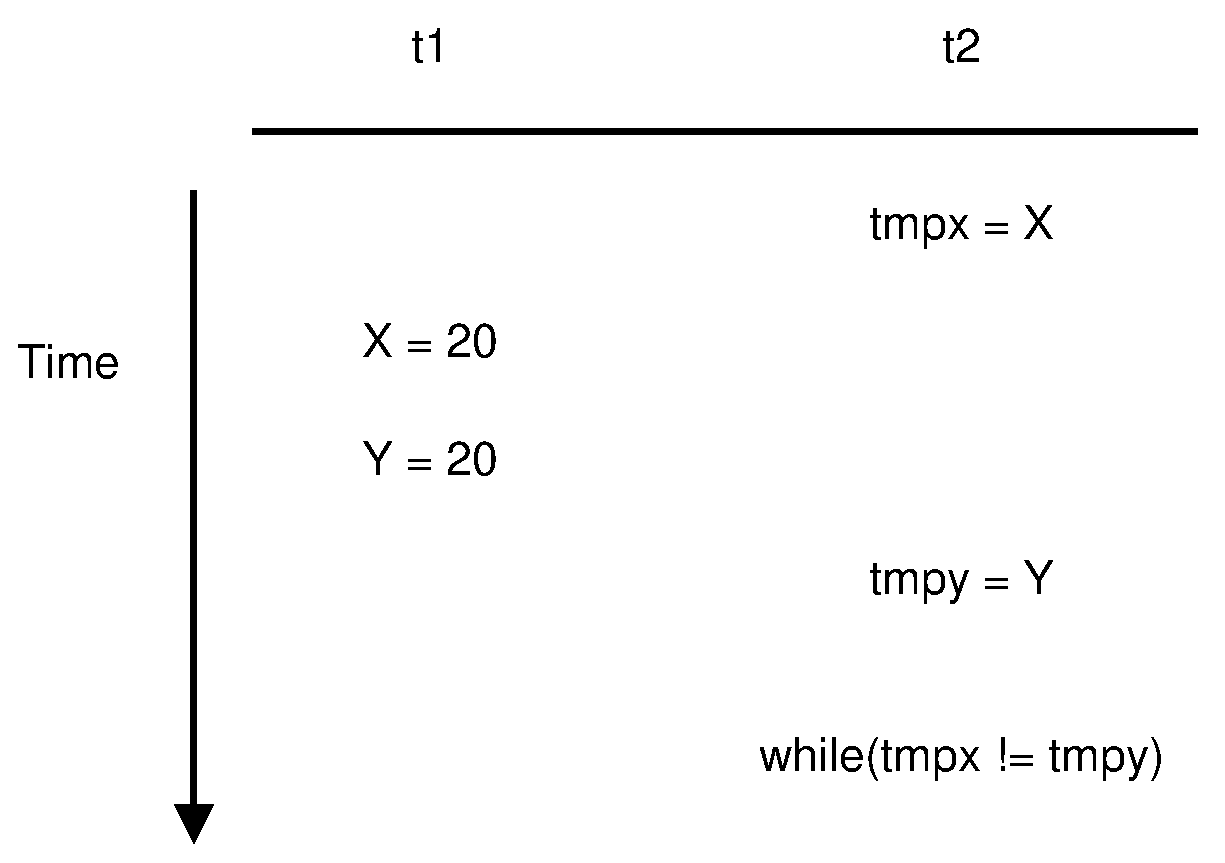
\includegraphics[width=0.65\textwidth]{\rootpath/worksheets/stm_requirements/figures/opacity_interleaving} 
 \caption{Opacity interleaving example}
\label{fig:opacity_interleaving}
\end{figure}

As opacity bolster the simplicity of using \ac{STM}, it is required for \stmname. This will positively impact the level of abstraction, readability and writability.

\section{Summary of Requirements}
In the following section, the requirements will be summarized in order to get a clear overview of properties \stmnamesp must have. 

The granularity of tracking \stmnamesp will provide, is on the variable level. That is, the assignments to variables will be tracked, however side-effects to the referenced object will not. Tracking the internals of an object will require the objects field to be marked as transactional variables. A transaction scope can be defined by a syntax extension provided in \stmname. Transactions in \stmnamesp is under the guarantee of strong atomicity, providing isolation between transactional and non-transactional code. As the \ac{STM} system does not track side-effects, use of immutable objects is promoted. Exceptions occurring inside a transaction will be propagated out of the transaction, in if the transaction is able to commit. Thus transactions will only be used for synchronization, not recovery of state. All irreversible actions, as mentioned in \bsref{subsec:irreversible} are discouraged. \stmnamesp must facilitate conditional synchronization, this is done by supplying the \bscode{retry} and \bscode{orElse} constructs. Nesting is allowed in \stmnamesp under closed nesting semantics, which strikes a balance between minimizing aborts and ensuring simple semantics for nested transactions. Lastly, opacity will be required for \stmnamesp, as this correctness criteria will bolster the simplicity of the \ac{STM} system.
\worksheetend